\section{Análise no Tempo Contínuo}

\begin{frame}{Comportamento Dinâmico do Sistema}
  \begin{figure}
    \centering
    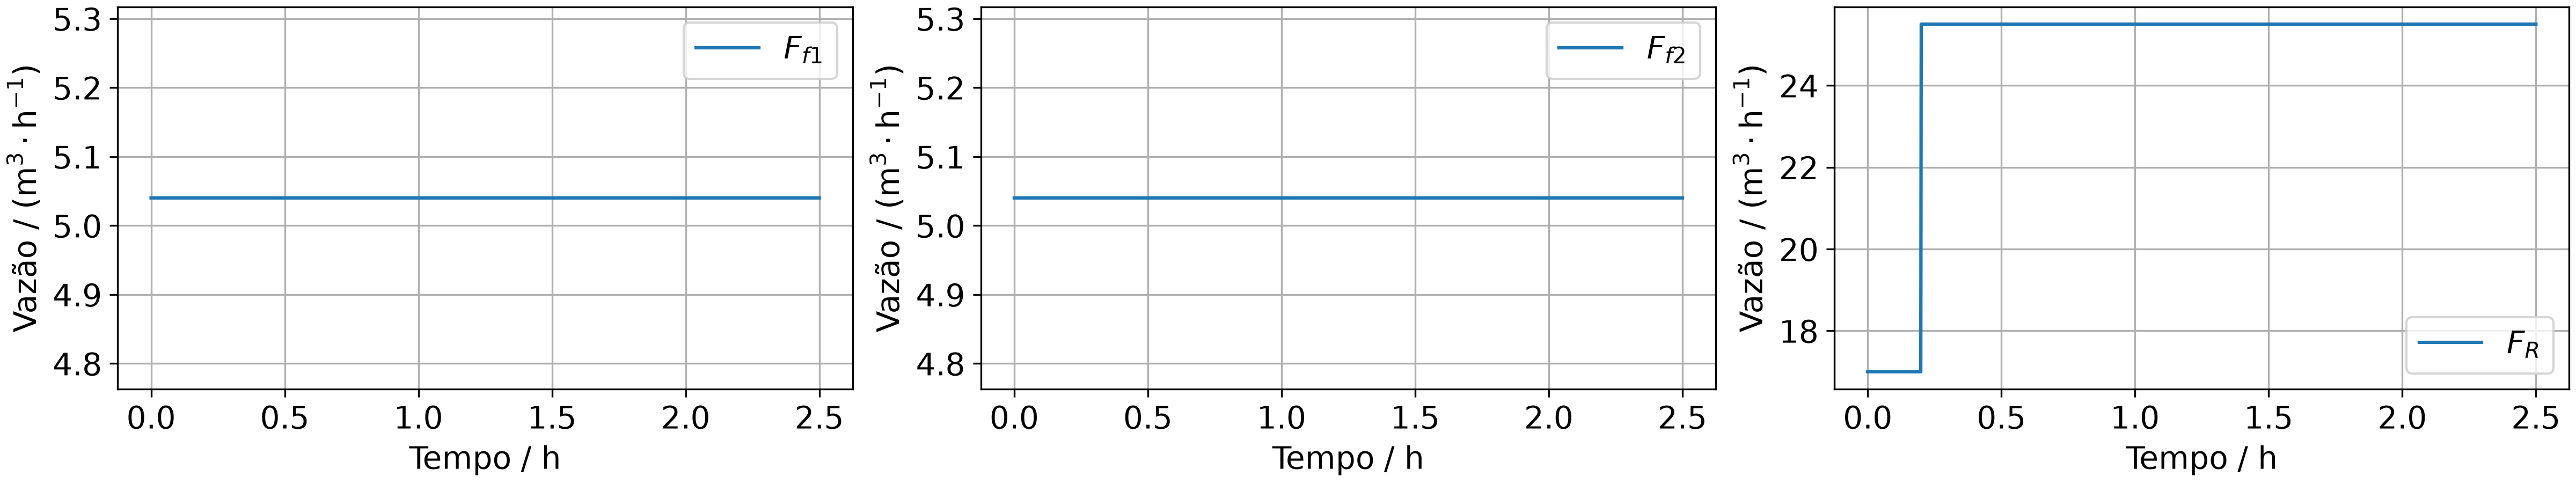
\includegraphics[width=0.8\linewidth]{../../figures/nonlinear/step-FR-inputs.png}
    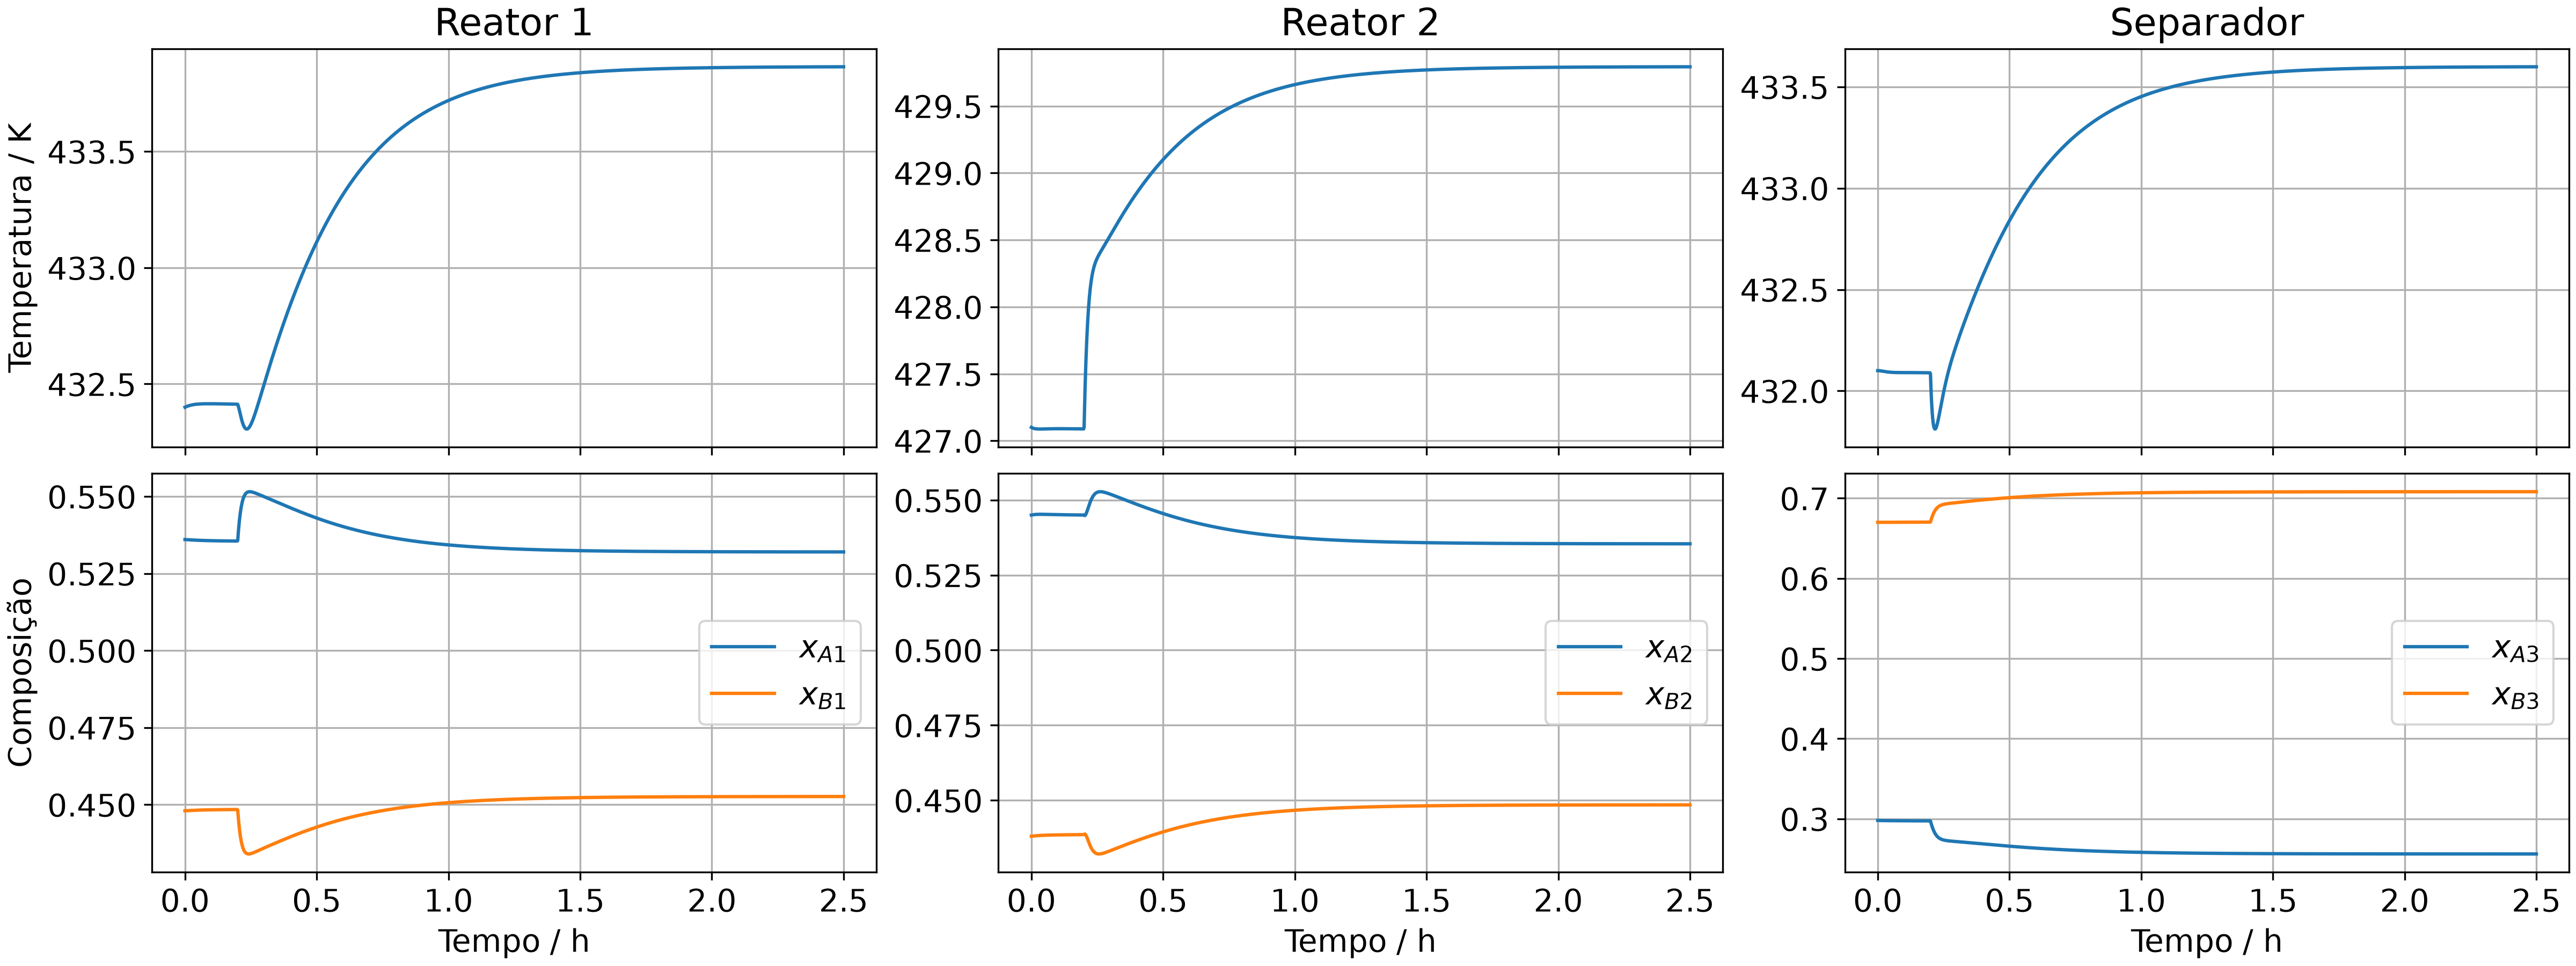
\includegraphics[width=0.8\linewidth]{../../figures/nonlinear/step-FR-outputs.png}
    \caption{Entradas e saídas do sistema para um degrau em $F_R$.}
  \end{figure}
\end{frame}

\begin{frame}
  \newcommand{\ua}{$\uparrow$}
  \newcommand{\da}{$\downarrow$}
  \newcommand{\nz}{$\approx 0$}
  \newcommand{\nm}{$^{\text{nm}}$}
  \begin{columns}
    \column{0.6\textwidth}
    \small
    \begin{table}[h!]
      \centering
      \begin{tabular}{c|ccccccc}
        \hline
        $\mathbf{y} / \mathbf{u}$ & $F_{f1}$ & $F_{f2}$ & \textcolor{red}{$F_R$}  \\
        \hline
        $T_1$                     & \da      & \da      & \textcolor{red}{\da\ua} \\
        $x_{A1}$                  & \ua      & \ua      & \textcolor{red}{\ua\da} \\
        $x_{B1}$                  & \da      & \da      & \textcolor{red}{\da\ua} \\
        % $x_{C1}$ & \da & \da & \textcolor{red}{\da\da\nz    \\
        \hline
        $T_2$                     & \da      & \da      & \textcolor{red}{\ua}    \\
        $x_{A2}$                  & \ua      & \ua      & \textcolor{red}{\ua\da} \\
        $x_{B2}$                  & \da      & \da      & \textcolor{red}{\da\ua} \\
        % $x_{C2}$ & \da & \da & \textcolor{red}{\da\da\nz}    \\
        \hline
        $T_3$                     & \da      & \da      & \textcolor{red}{\da\ua} \\
        $x_{A3}$                  & \ua      & \ua      & \textcolor{red}{\da}    \\
        $x_{B3}$                  & \da      & \da      & \textcolor{red}{\ua}    \\
        % $x_{C3}$ & \da & \da & \textcolor{red}{\ua\nm\nz}   \\
        \hline
      \end{tabular}
      \caption{Interação entre entradas e estados.}
    \end{table}
    \column{0.4\textwidth}
    \begin{itemize}
      \item \ua: ganho positivo;
      \item \da: ganho negativo;
      \item \da\ua: ganho positivo com resposta inversa;
      \item \ua\da: ganho negativo com resposta inversa;
            % \item \ua\ua: ganho positivo com sobressinal;
            % \item \da\da: ganho negativo com sobressinal;
            % \item \nm: resposta não monotônica;
            % \item \nz: ganho muito pequeno.
    \end{itemize}
  \end{columns}
\end{frame}

\begin{frame}{Linearização}
  O modelo foi linearizado em torno do ponto de operação de
  \citeonline{pourkargar_2017}, permitindo sua análise por técnicas lineares.
  \begin{columns}[T]
    \column{0.5\textwidth}
    \begin{table}
      \caption{Entradas $u_{ss}$}
      \begin{tabular}{lll}
        \hline
        Variável & Valor   & Unidade \\
        \hline
        $F_{f1}$ & 5{,}04  & m³/h    \\
        $F_{f2}$ & 5{,}04  & m³/h    \\
        $F_R$    & 17{,}00 & m³/h    \\
        \hline
      \end{tabular}
    \end{table}
    \column{0.5\textwidth}
    \begin{table}
      \caption{Estados $y_{ss}$}
      \begin{tabular}{lll}
        \hline
        Variável & Valor   & Unidade \\
        \hline
        $T_1$    & 432{,}4 & K       \\
        $T_2$    & 427{,}1 & K       \\
        $T_3$    & 432{,}1 & K       \\
        $x_{A1}$ & 0{,}536 & --      \\
        $x_{B1}$ & 0{,}448 & --      \\
        $x_{A2}$ & 0{,}545 & --      \\
        $x_{B2}$ & 0{,}438 & --      \\
        $x_{A3}$ & 0{,}298 & --      \\
        $x_{B3}$ & 0{,}670 & --      \\
        \hline
      \end{tabular}
    \end{table}
  \end{columns}
\end{frame}

\begin{frame}{Comparação entre o modelo linear e não linear}
  \begin{columns}
    \column{0.5\textwidth}
    \begin{figure}
      \centering
      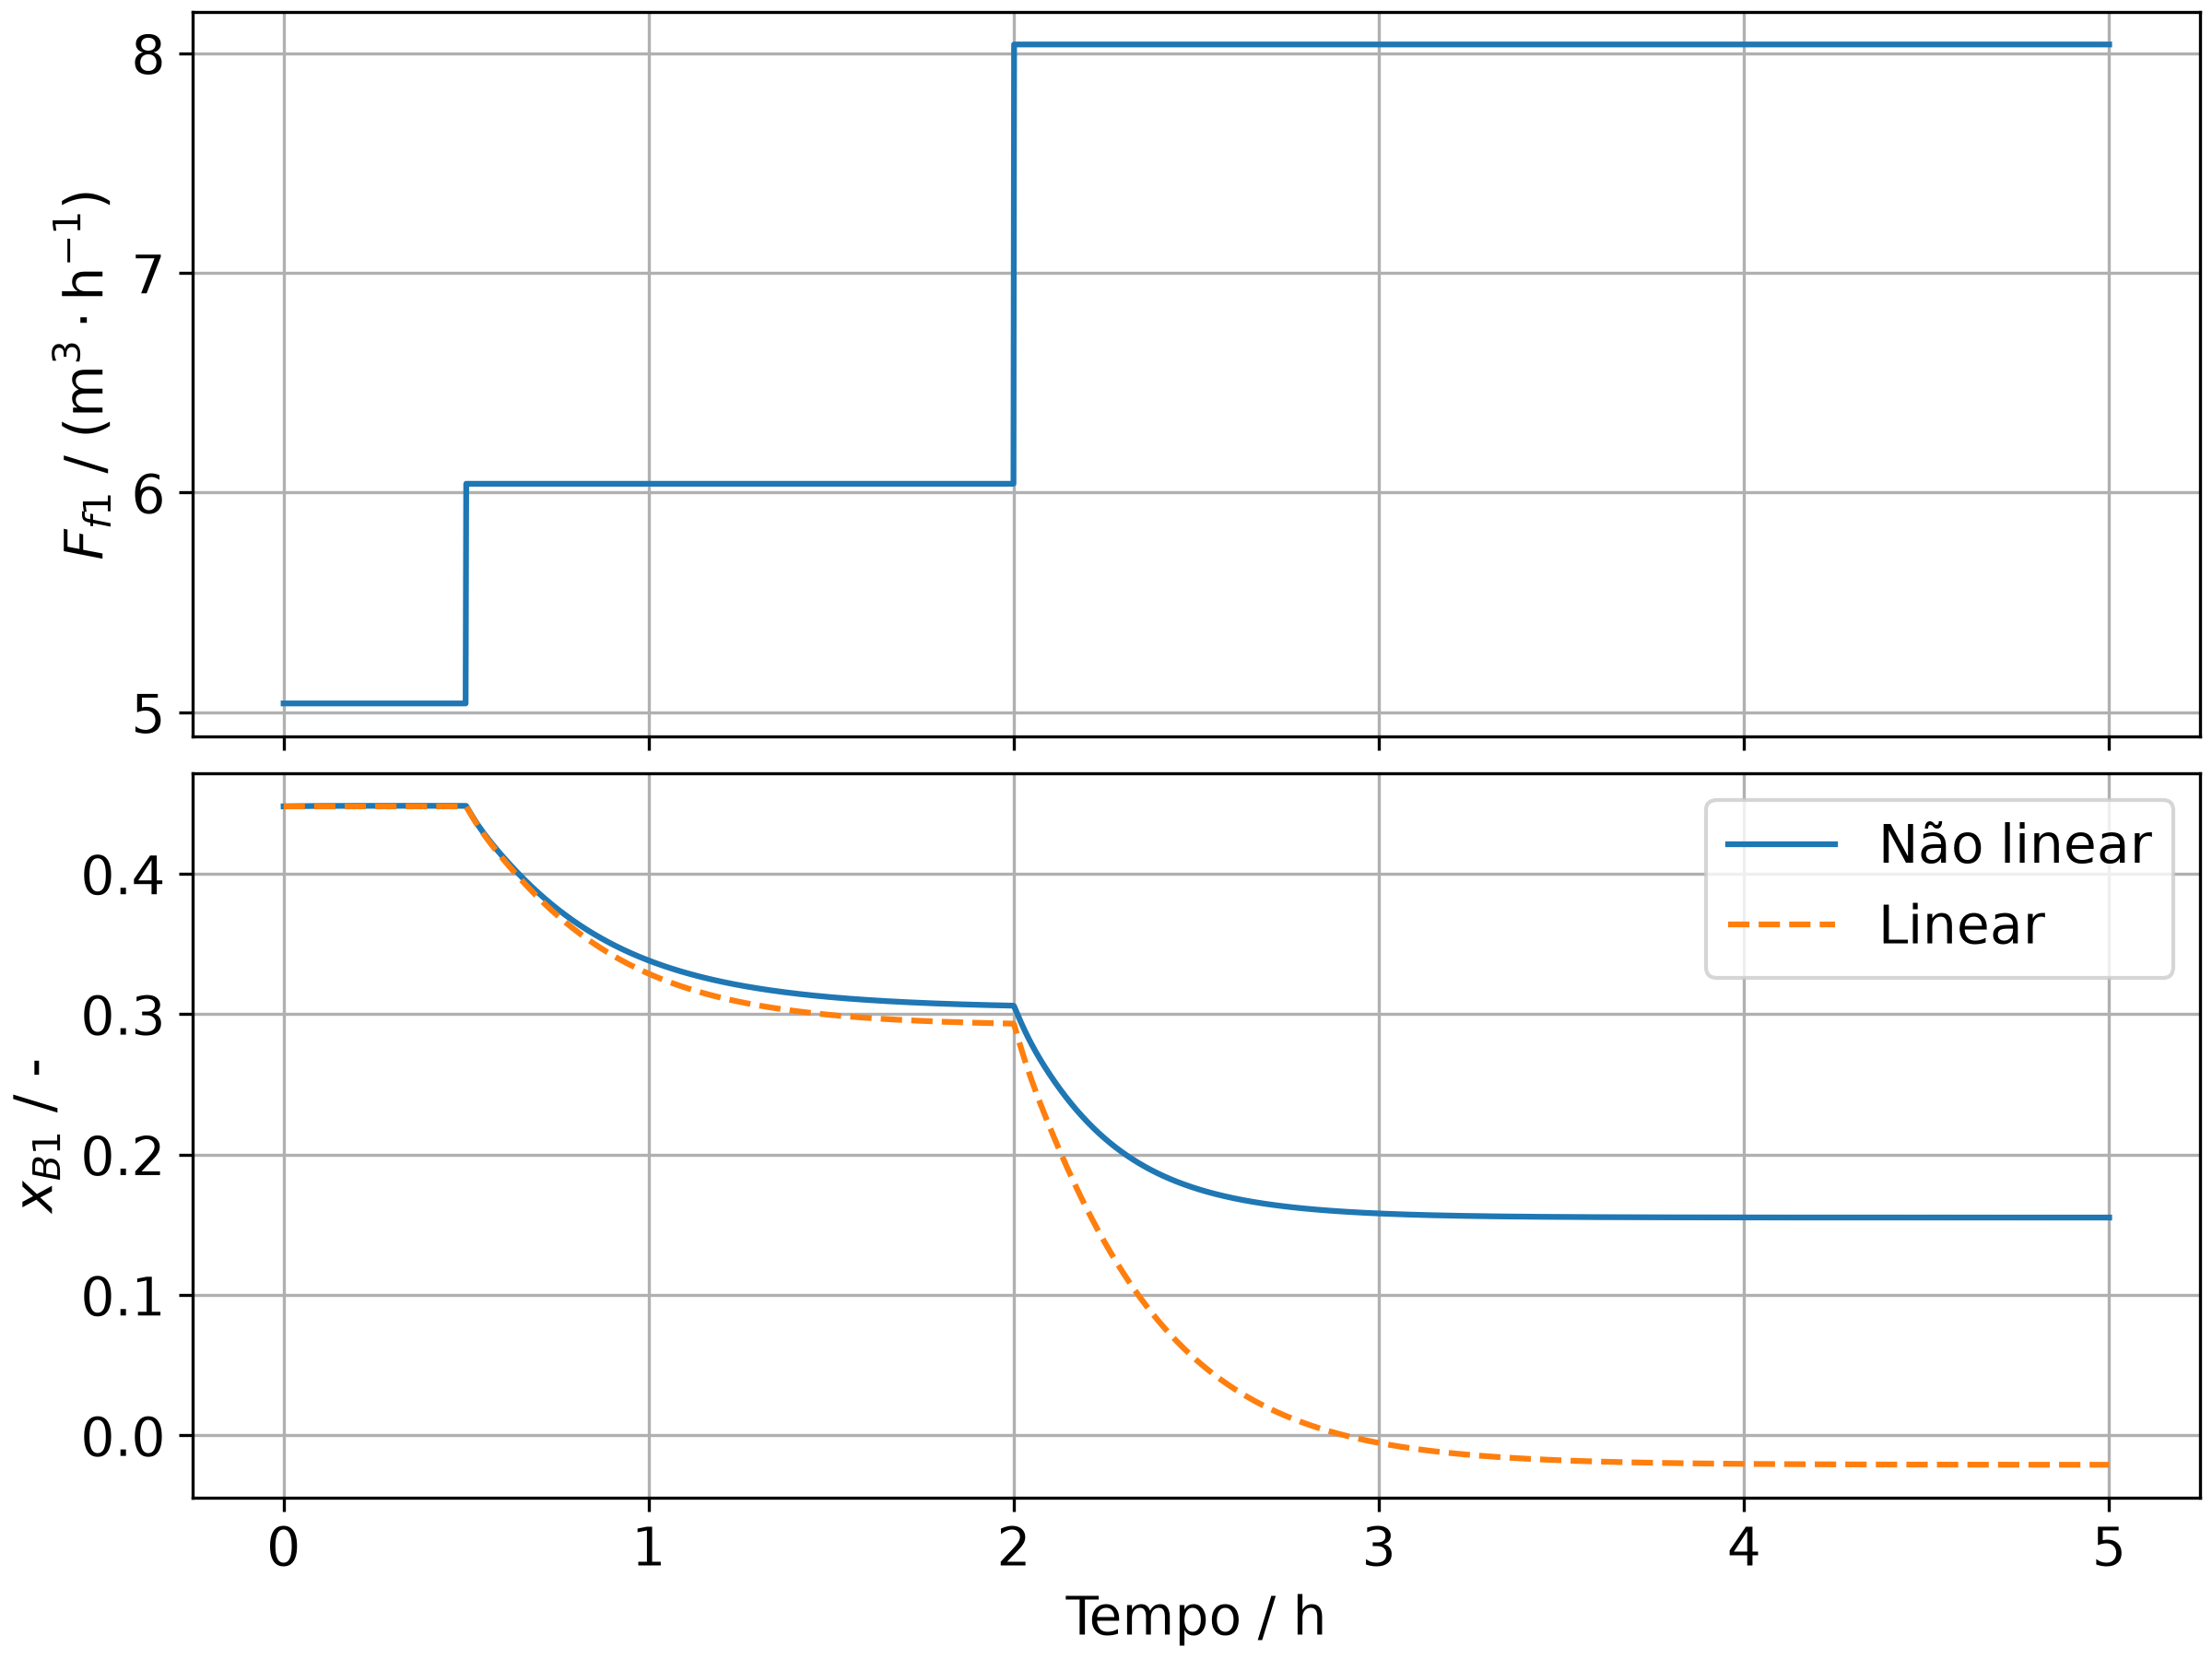
\includegraphics[width=\textwidth]{../../figures/linear_vs_nonlinear/xB1_Ff1.png}
      \caption{Resposta da variável $x_{B1}$ a perturbações na entrada $F_{f1}$.}
    \end{figure}
    \column{0.5\textwidth}
    \begin{itemize}
      \item Boa concordância próxima ao ponto de linearização.
      \item As respostas divergem à medida que o sistema se afasta desse ponto.
      \item E o modelo linear prevê $x_{B1}<0$, sem significado físico, mostrando que a linearização é válida apenas localmente.
    \end{itemize}
  \end{columns}
\end{frame}
